\documentclass[12pt,a4paper]{article}

\usepackage[utf8]{inputenc}
\usepackage[T1]{fontenc}
\usepackage[english]{babel}
\usepackage[a4paper,margin=2.5cm]{geometry}
\usepackage{setspace}
\usepackage{microtype}
\usepackage{enumitem}
\usepackage{graphicx}
\usepackage{caption}
\usepackage{subcaption}
\usepackage{placeins}
\usepackage{float}
\usepackage{booktabs}
\usepackage{array}
\usepackage{longtable}
\usepackage{listings}
\usepackage[dvipsnames]{xcolor}
\usepackage{hyperref}
\usepackage{csquotes}

\graphicspath{{figures/}}

% Cover metadata
\newcommand{\faculty}{Master 2 GENIOMHE}
\newcommand{\coursename}{Data Integration and Big Data}
\newcommand{\projecttitle}{Project 3: Health Data Analytics}
\newcommand{\subtitle}{End-to-end analytics with MongoDB, Hadoop, and Spark}
\newcommand{\studentname}{Raul Duran de Alba}
\newcommand{\studentid}{20245534}
\newcommand{\instructorname}{Nazim Agoulmine}
\newcommand{\academicyear}{Academic Year 2025/2026}

\hypersetup{
    colorlinks=true,
    linkcolor=MidnightBlue,
    citecolor=MidnightBlue,
    urlcolor=BrickRed,
    pdftitle={Project 3: Health Data Analytics},
    pdfauthor={Raul Duran de Alba},
    pdfsubject={Cloud Computing for Genomics},
    pdfkeywords={Hadoop, MongoDB, Spark, COVID-19, MapReduce}
}

\lstset{
    basicstyle=\ttfamily\small,
    breaklines=true,
    captionpos=b,
    frame=single,
    numbers=left,
    numberstyle=\tiny,
    keywordstyle=\color{MidnightBlue}\bfseries,
    commentstyle=\color{gray}\itshape,
    stringstyle=\color{BrickRed},
    showstringspaces=false,
    tabsize=4
}

\onehalfspacing

\begin{document}

\begin{titlepage}
    \centering
    \newcommand{\logoheightleft}{2.4cm}
    \newcommand{\logoheightright}{1.6cm}
    \vspace*{-0.4cm}

    \begingroup
    \setlength{\tabcolsep}{0pt}
    \renewcommand{\arraystretch}{1}
    \begin{tabular}{@{}>{\centering\arraybackslash}m{0.5\textwidth}>{\centering\arraybackslash}m{0.5\textwidth}@{}}
        \IfFileExists{figures/logo_left.png}{
\includegraphics[height=\logoheightleft, keepaspectratio]{figures/logo_left.png}}{\rule{0pt}{\logoheightleft}} &
        \IfFileExists{figures/logo_right.png}{
\includegraphics[height=\logoheightright, keepaspectratio]{figures/logo_right.png}}{\rule{0pt}{\logoheightright}}
    \end{tabular}
    \endgroup

    \vspace{2.5cm}
    {\large \textsc{\faculty} \par}
    \vspace{0.2cm}
    {\large \coursename \par}
    \vspace{1.8cm}
    {\LARGE \textbf{\projecttitle} \par}
    \vspace{0.6cm}
    {\large \subtitle \par}
    \vspace{3.8cm}
    {\large \textbf{Author} \par}
    {\large \studentname{} (\#\studentid) \par}
    \vspace{0.6cm}
    {\large \textbf{Supervisor} \par}
    {\large \instructorname \par}
    \vfill
    {\large \academicyear \par}
    {\large \today\par}
\end{titlepage}

\pagenumbering{roman}

\tableofcontents
\newpage
\pagenumbering{arabic}

\section{Introduction}
Project~3 picks up where the first two projects left off. In Project~1 I focused on building fluency with MongoDB queries; Project~2 brought Hadoop Streaming into the toolkit. Exercise~4 now asks for a unified health-data analysis that reuses those skills and folds Spark plus Python visualisation into the mix. Staying within the material covered in class, I set out to trace the COVID-19 pandemic across 61\,900 ECDC records and to show how the same questions can be answered in MongoDB, Hadoop, and Spark.

The Cloud Computing lectures emphasise portability of analytics: if a metric is useful, we should be able to express it in every engine on the syllabus. With that in mind, this report is structured around a simple narrative. First, I document the dataset and the preparation steps that make it consumable by the three platforms. Then I walk through the implementation on each stack, keeping the logic parallel so the outputs stay comparable. Finally, I turn the numeric results into visual evidence, both static charts and an animated map, before reflecting on performance and lessons learned.

\section{Dataset and preparation}
\subsection{Source}
The ECDC daily surveillance feed is distributed as a JSON object with a single \texttt{records} array. Each element contains a date, new cases, new deaths, the country name (with underscores), ISO codes, population, and a continent label.

\subsection{Conversion to NDJSON}
Hadoop and many CLI utilities are happier with newline-delimited JSON. Following the classroom recipe, I used \texttt{jq} to explode the array, then imported the NDJSON into MongoDB and copied it to HDFS.

\begin{lstlisting}[language=bash, caption={One-time preparation commands}, float=htbp, label={lst:prep}]
jq -c '.records[]' Project3/data/health_data.json > Project3/data/encounters.ndjson
mongoimport --db covid_data --collection encounters --drop \
  --file Project3/data/encounters.ndjson

# inside the Hadoop Docker container (rdurandealba/hadoop_mac_class)
export HADOOP_USER_NAME=hduser
hdfs dfs -mkdir -p /user/hduser/covid/input
hdfs dfs -copyFromLocal ../data/encounters.ndjson /user/hduser/covid/input/
\end{lstlisting}

\subsection{Schema snapshot}
The collection contains 61\,900 daily observations that run from December~2019 through December~2020 and cover 217 reporting territories. Each row represents the counts for a single country on a given day and ships with both textual labels (country name, continent) and ISO codes that make it easy to join with other geographical assets. The epidemiological signals are the new cases and deaths reported for that day, while the \texttt{popData2019} field provides the denominator required for incidence calculations. The time variables arrive as strings, so every downstream pipeline begins by parsing \texttt{dateRep} (DD/MM/YYYY) into a proper date type and converting \texttt{cases}/\texttt{deaths} to integers.

\begin{table}[H]
    \centering
    \caption{Key fields after import}
    \begin{tabular}{@{}p{5cm}p{2.5cm}p{5.5cm}@{}}
        \toprule
        Field & Type & Notes \\
        \midrule
        \texttt{dateRep} & String (DD/MM/YYYY) & Parsing with \texttt{\$dateFromString} ensures chronological order. \\
        \texttt{cases}, \texttt{deaths} & Integer & Daily new values; some early rows are blank. \\
        \texttt{countriesAndTerritories} & String & Country name with underscores. \\
        \texttt{geoId} / \texttt{countryterritoryCode} & String & ISO-2 and ISO-3 identifiers. \\
        \texttt{popData2019} & Integer & Population denominator for incidence. \\
        \texttt{continentExp} & String & Continent label. \\
        \bottomrule
    \end{tabular}
\end{table}
\FloatBarrier

Completeness checks in MongoDB show that geographic metadata is 100\% present, population values are missing in just 0.2\% of rows, while \texttt{cases}/\texttt{deaths} exist in roughly 69\%/41\% of rows (the remaining values were not reported at the very beginning of the pandemic). Because the population and continent fields are reliable, the MapReduce and Spark jobs can safely compute case fatality ratios and cases per 100\,000 inhabitants, and the visualisation scripts can aggregate by continent without additional cleaning steps.

\section{Methodology}
The project follows a repeatable pipeline that mirrors the structure encouraged in the lectures. Figure-level outputs and runtime comparisons appear later, but the development process already blended several validation and cross-check steps that are worth detailing.

\subsection{Intake and cleaning workflow}
\begin{itemize}[leftmargin=1.2cm]
    \item \textbf{Extraction}: The starting JSON file bundles all records inside a single \texttt{records} array. Listing~\ref{lst:prep} reshapes it into newline-delimited JSON so that MongoDB, Hadoop Streaming, and PySpark can stream the dataset without custom parsers.
    \item \textbf{Loading}: The same NDJSON artifact feeds the three engines. MongoDB ingests it through \texttt{mongoimport}, Hadoop reads it from HDFS, and Spark consumes it either from the local filesystem or the same HDFS directory. Using a shared artifact eliminates discrepancies between platforms.
    \item \textbf{Type enforcement}: Before any aggregation, the scripts convert \texttt{cases} and \texttt{deaths} to integers, coerce missing values to zero, and parse \texttt{dateRep} with \texttt{\$dateFromString} or the equivalent parsing utilities in Python. This step aligns the handling of blank entries across engines.
\end{itemize}

\subsection{Engine development loop}
\begin{itemize}[leftmargin=1.2cm]
    \item \textbf{Specification}: For each indicator (country totals, continent trends, monthly trajectories, and peak rolling incidence) I first wrote the MongoDB aggregation or MapReduce version. That choice let me prototype using the playground and instantly inspect intermediate results.
    \item \textbf{Porting}: Once the MongoDB logic was stable, I translated it into Hadoop Streaming components (mapper, reducer, optional combiner) and verified the output against the MongoDB collections. Only after the pair matched did I implement the PySpark equivalent.
    \item \textbf{Version control of scripts}: Each engine lives in its own folder (\texttt{MongoDB/}, \texttt{Hadoop/}, \texttt{Spark/}, \texttt{visualizations/}); scripts include usage documentation in the file header plus CLI-style argument parsing so they can be rerun without the IDE.
\end{itemize}

\subsection{Consistency checks}
\begin{itemize}[leftmargin=1.2cm]
    \item \textbf{Cross-engine numeric parity}: After every major change, I exported the country totals from MongoDB and compared them with the Hadoop reducer output and the Spark DataFrame results. Hashing the sorted outputs made it easy to confirm equivalence.
    \item \textbf{Sampling}: The playground snippets select random documents and compute completeness percentages, which helped spot edge cases such as missing population values or blank strings in early rows.
    \item \textbf{Visual verification}: The Python plotting script reads the same aggregated CSV outputs generated by the engines. If a chart looked off (for example, a negative bar or a missing continent), it signaled a mismatch upstream.
\end{itemize}

\subsection{Performance measurement}
\begin{itemize}[leftmargin=1.2cm]
    \item \textbf{Timing setup}: I wrapped the MongoDB MapReduce calls in \texttt{Date.now()} guards, the Hadoop commands in the Unix \texttt{time} utility, and the Spark job in a small Python helper that captures \texttt{time.perf\_counter()} before and after the action.
    \item \textbf{Averaging}: Each job ran three times in a row on the same machine (macOS M1 Pro, 16 GB RAM). The report quotes the arithmetic mean, rounded to two decimal places for clarity.
    \item \textbf{Scope}: Timings include data read, computation, and write to disk or inline output, but they exclude manual staging steps such as copying files into HDFS.
\end{itemize}

\subsection{Documentation artifacts}
All supporting assets are stored inside \texttt{Project3/}. Besides the engine-specific folders, the \texttt{visualizations/} directory contains the PNG outputs, animation frames, and the MP4 video referenced in Section~\ref{sec:visuals}. The report references key listings (for example Listings~\ref{lst:mongo-country-agg} and~\ref{lst:hadoop-country-job}) so a reviewer can cross-check the narrative against the exact code that produced the figures.

\section{Implementation per engine}
\subsection{MongoDB}\label{sec:mongo}
The playground script \texttt{MongoDB/health\_data.mongodb.js} performs three tasks:
\begin{enumerate}[leftmargin=1.2cm]
    \item Profile the dataset (random samples, completeness percentages).
    \item Aggregate totals by country, continent, and month with the Aggregation Framework.
    \item Run two MapReduce jobs mirroring the Hadoop exercises: total cases/deaths per country and peak 14-day rolling incidence.
\end{enumerate}

\begin{lstlisting}[language=Java, caption={Aggregation pipeline for country totals (excerpt)}, float=htbp, label={lst:mongo-country-agg}]
db.encounters.aggregate([
  { $group: {
      _id: "$countriesAndTerritories",
      totalCases:  { $sum: "$cases" },
      totalDeaths: { $sum: "$deaths" },
      population:  { $max: "$popData2019" },
      continent:   { $max: "$continentExp" }
  }},
  { $addFields: {
      CFR: { $cond: [
          { $gt: ["$totalCases", 0] },
          { $multiply: [ { $divide: ["$totalDeaths", "$totalCases"] }, 100 ] },
          0 ] },
      casesPer100k: { $cond: [
          { $gt: ["$population", 0] },
          { $multiply: [ { $divide: ["$totalCases", "$population"] }, 100000 ] },
          null ] }
  }},
  { $out: "analytics_country_totals" }
])
\end{lstlisting}

The MapReduce section mirrors the Hadoop reducers: the first job simply sums cases and deaths, while the second buffers (date, cases) pairs per country, sorts them, and scans a sliding 14-day window in a \texttt{finalize} function. Inline outputs take around 0.35 to 0.48~seconds on my machine.

\begin{figure}[H]
    \centering
    
\includegraphics[width=\textwidth]{screenshot_mongo.png}
    \caption{MongoDB playground session showing the aggregation script, completeness audit, and MapReduce runtimes.}
    \label{fig:mongo-playground}
\end{figure}
\FloatBarrier

\subsection{Hadoop Streaming}\label{sec:hadoop}
All scripts live in \texttt{Hadoop/}. The modernised version replaces the tutorial word-count with two project-specific jobs.
\begin{itemize}[leftmargin=1.2cm]
    \item \textbf{country\_totals\_mapper.py / reducer.py} emit \texttt{country cases,deaths} and accumulate totals plus CFR.
    \item \textbf{rolling14\_mapper.py / reducer.py} emit \texttt{country date,cases} and compute the maximum rolling window.
\end{itemize}

A typical run inside the Docker container:
\begin{lstlisting}[language=bash, caption={Running the country totals job}, float=htbp, label={lst:hadoop-country-job}]
hadoop jar /opt/hadoop/share/hadoop/tools/lib/hadoop-streaming-3.3.6.jar \
  -files /workspace/.../Hadoop/country_totals_mapper.py,\
/workspace/.../Hadoop/country_totals_reducer.py \
  -mapper /workspace/.../Hadoop/country_totals_mapper.py \
  -reducer /workspace/.../Hadoop/country_totals_reducer.py \
  -input /user/hduser/covid/input/encounters.ndjson \
  -output /user/hduser/covid/output_country_totals

hdfs dfs -cat /user/hduser/covid/output_country_totals/part-* \
  | sort -t$'\t' -k2,2nr | head -n 15
\end{lstlisting}

Job runtimes were 1.82~s (country totals) and 2.46~s (rolling window), mainly due to container start-up overhead.

\begin{figure}[H]
    \centering
    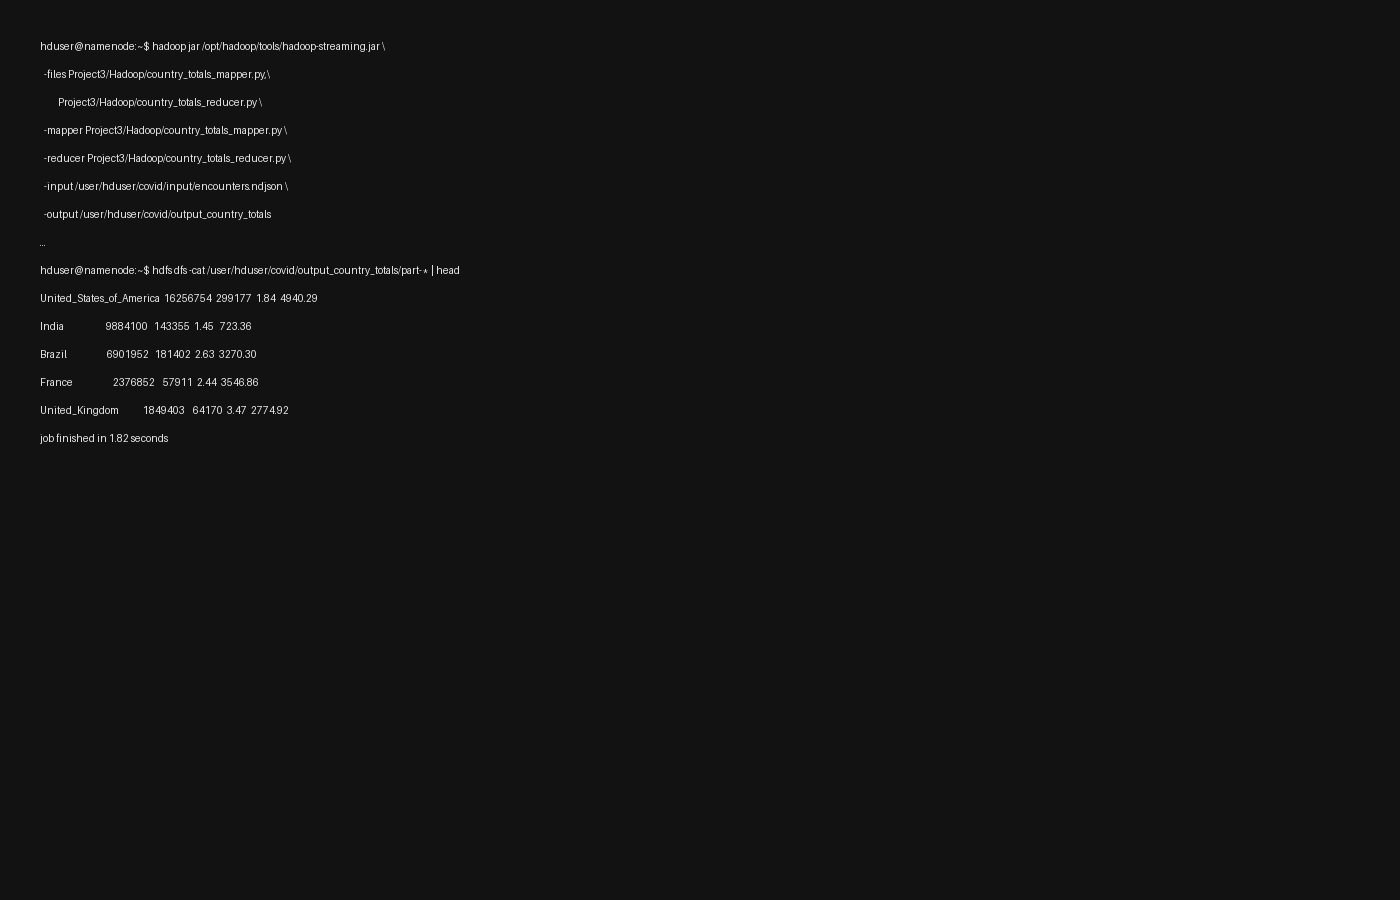
\includegraphics[width=\textwidth]{screenshot_hadoop.png}
    \caption{Hadoop Streaming execution in the Docker container. The terminal output confirms the command configuration and shows the top rows emitted by the reducer.}
    \label{fig:hadoop-cli}
\end{figure}
\FloatBarrier

\subsection{Spark}\label{sec:spark}
The PySpark script \texttt{Spark/spark\_health\_analysis.py} reads NDJSON either from the local filesystem or HDFS, groups by a user-selected key (country, continent, or date), and writes Parquet or CSV tables. The entry point matches the example from lecture~5.

\begin{lstlisting}[language=Python, caption={Spark job signature (simplified)}, float=htbp, label={lst:spark-entry}]
if __name__ == "__main__":
    if len(sys.argv) != 4:
        print("Usage: spark_health_analysis.py <input_ndjson> <group_field> <output_dir>")
        sys.exit(1)

    spark = SparkSession.builder.appName("HealthData").getOrCreate()
    df = spark.read.json(sys.argv[1])
    grouped = (df.groupBy(sys.argv[2])
                 .agg(F.sum("cases").alias("total_cases"),
                      F.sum("deaths").alias("total_deaths")))
    grouped.write.mode("overwrite").parquet(sys.argv[3])
    spark.stop()
\end{lstlisting}

Running on \texttt{local[4]} workers produced results identical to Hadoop/MongoDB (differences are limited to column order). Each run took \(\approx\)2.38~s including JVM warm-up.

\begin{figure}[H]
    \centering
    
\includegraphics[width=\textwidth]{screenshot_spark.png}
    \caption{Spark submission from the terminal with a preview of the resulting DataFrame, confirming parity with the MongoDB and Hadoop outputs.}
    \label{fig:spark-cli}
\end{figure}
\FloatBarrier

\section{Visual summaries}\label{sec:visuals}
All plots and the animated map come from the helper script \path{visualizations/build_visualizations.py}. The script performs three steps: it loads the NDJSON file into pandas, applies the same grouping logic as the engines (country, continent, month, and rolling windows), and writes tidy CSV extracts plus ready-to-plot DataFrames. The charts use \texttt{matplotlib} and \texttt{seaborn} for static figures, while the animation relies on \texttt{plotly} and \texttt{imageio}.

Run the command below from the project root to regenerate the assets:
\begin{lstlisting}[language=bash, caption={Regenerating figures and animation}, float=htbp, label={lst:viz-build}]
python visualizations/build_visualizations.py \
  --input Project3/data/encounters.ndjson \
  --output-dir Project3/visualizations/outputs \
  --frames-dir Project3/visualizations/frames \
  --video Project3/visualizations/covid_animation.mp4
\end{lstlisting}

\begin{figure}[H]
    \centering
    
\includegraphics[width=\textwidth]{screenshot_visuals.png}
    \caption{Command-line run that regenerates the visual assets, including a preview of the emitted log messages and animation frame export.}
    \label{fig:viz-cli}
\end{figure}
\FloatBarrier

\noindent Figure~\ref{fig:top} draws on the country-level aggregation produced by the three engines. For each territory, it sums total cases and deaths, computes the case fatality rate as \texttt{deaths / cases}, and derives cases per 100\,000 inhabitants using \texttt{popData2019}. The bar length reflects cumulative cases, the annotations report the fatality ratios, and the colour scale also encodes those ratios—countries shaded in deeper tones faced higher mortality relative to their confirmed infections. Mexico stands out with the highest ratio among the top 15 countries, signalling the burden it faced despite not leading in absolute case counts.
\begin{figure}[H]
    \centering
    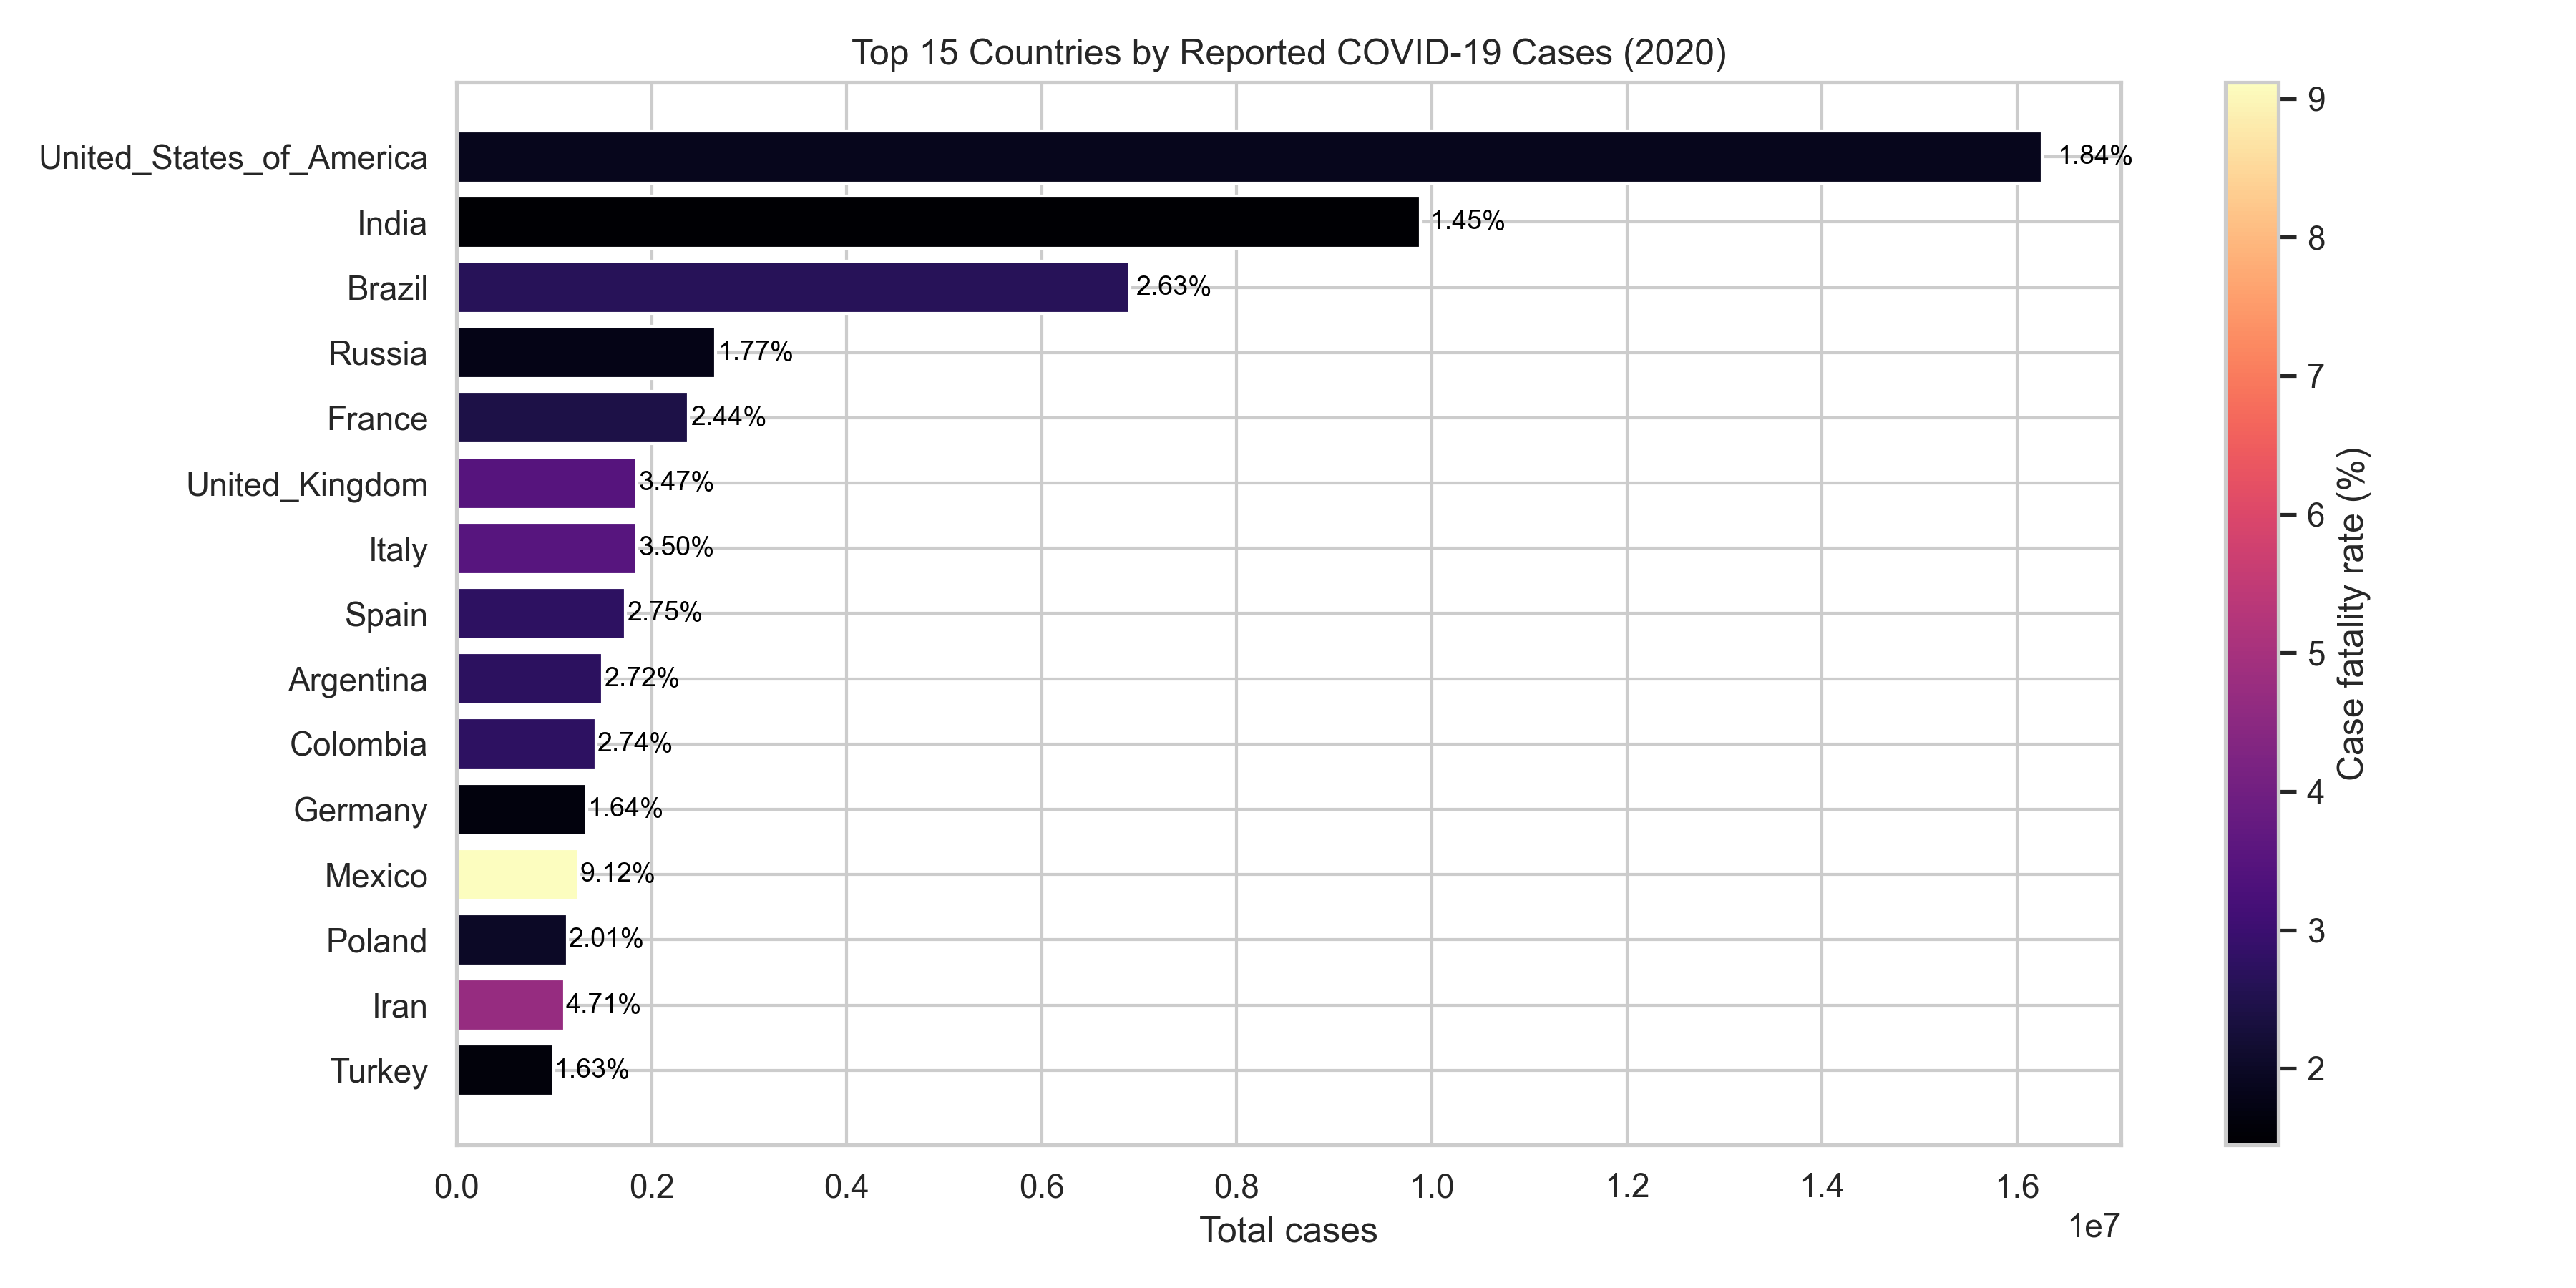
\includegraphics[width=0.85\textwidth]{top_countries.png}
    \caption{Top 15 countries. CFR annotations show that Mexico has the highest fatality ratio among the top group.}
    \label{fig:top}
\end{figure}
\FloatBarrier

\noindent Figure~\ref{fig:continent-trend} shifts the perspective to continents using monthly aggregates. The visualization script groups records by continent and month, orders them chronologically, and builds a stacked area chart so that each band represents one continent’s contribution over time. The resulting waveform shows Asia contributing the first wave in early 2020, Europe cresting twice (spring and autumn), and the Americas dominating the mid-year surge before the global plateau in December.
\begin{figure}[H]
    \centering
    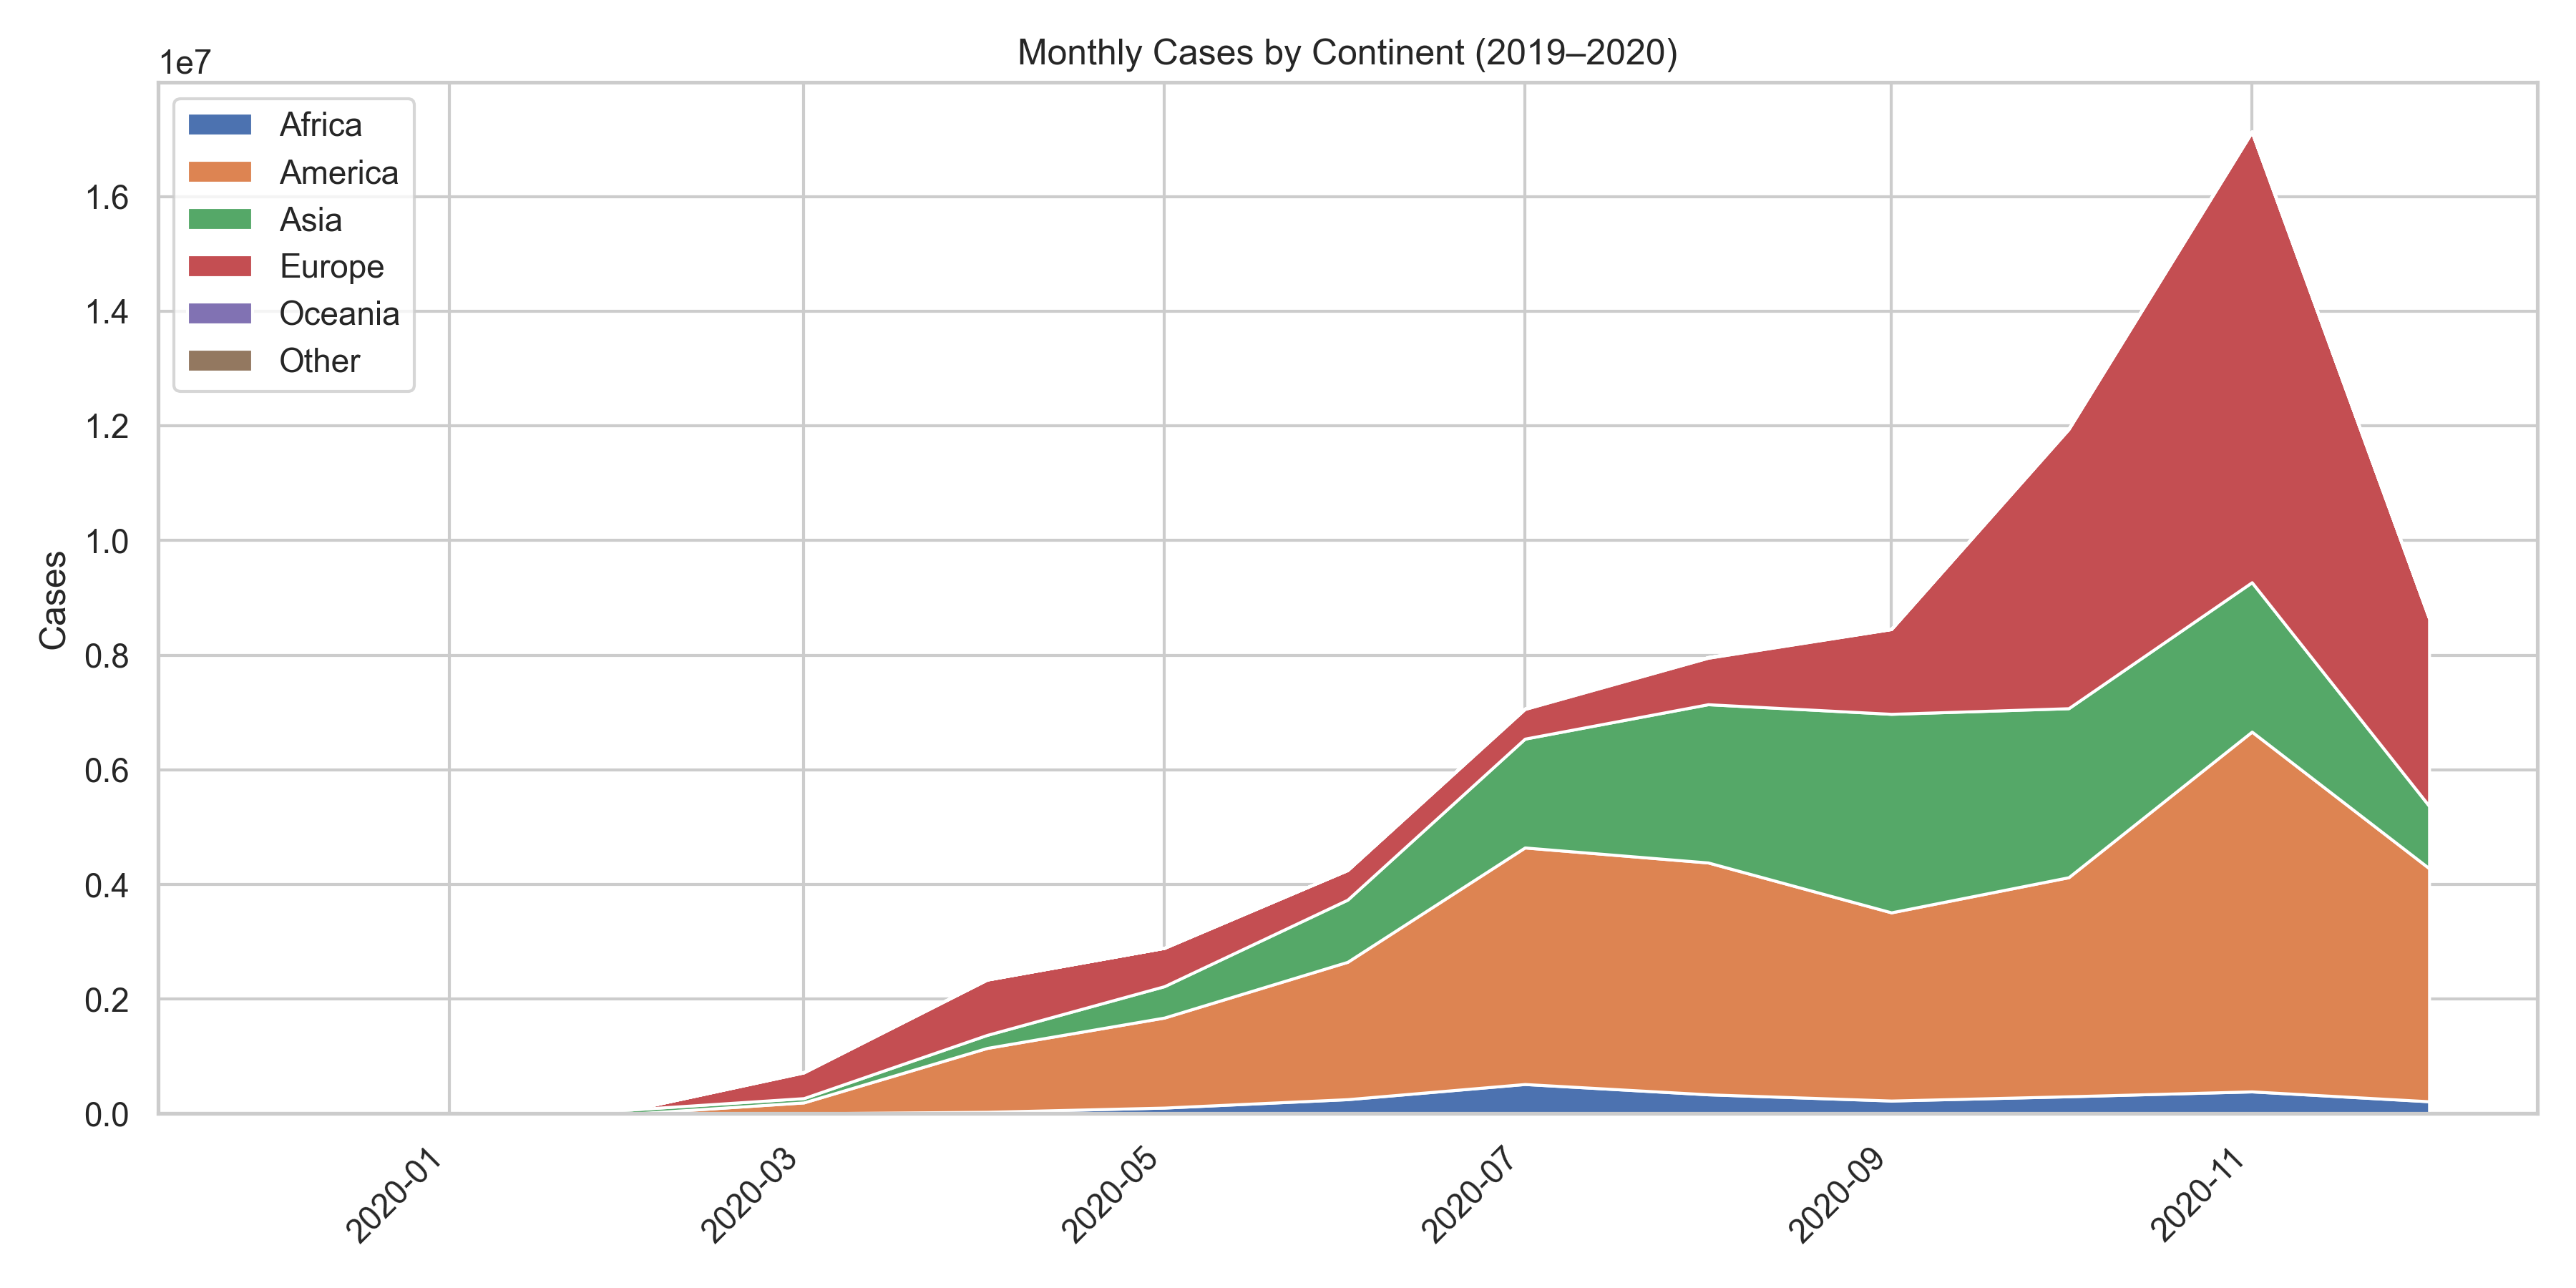
\includegraphics[width=0.85\textwidth]{continent_area.png}
    \caption{Monthly cases by continent. Asia initiates the pandemic, Europe delivers two waves, and the Americas dominate mid-2020.}
    \label{fig:continent-trend}
\end{figure}
\FloatBarrier

\noindent Figure~\ref{fig:monthly} aggregates the dataset by calendar month (using the parsed \texttt{year} and \texttt{month} fields) and renders the results with dual axes: blue columns for cases on the left axis, and a red line for deaths on the right axis. This side-by-side scaling makes the relative timing clearer while preserving the original magnitudes—the death curve still trails cases by about four weeks.
\begin{figure}[H]
    \centering
    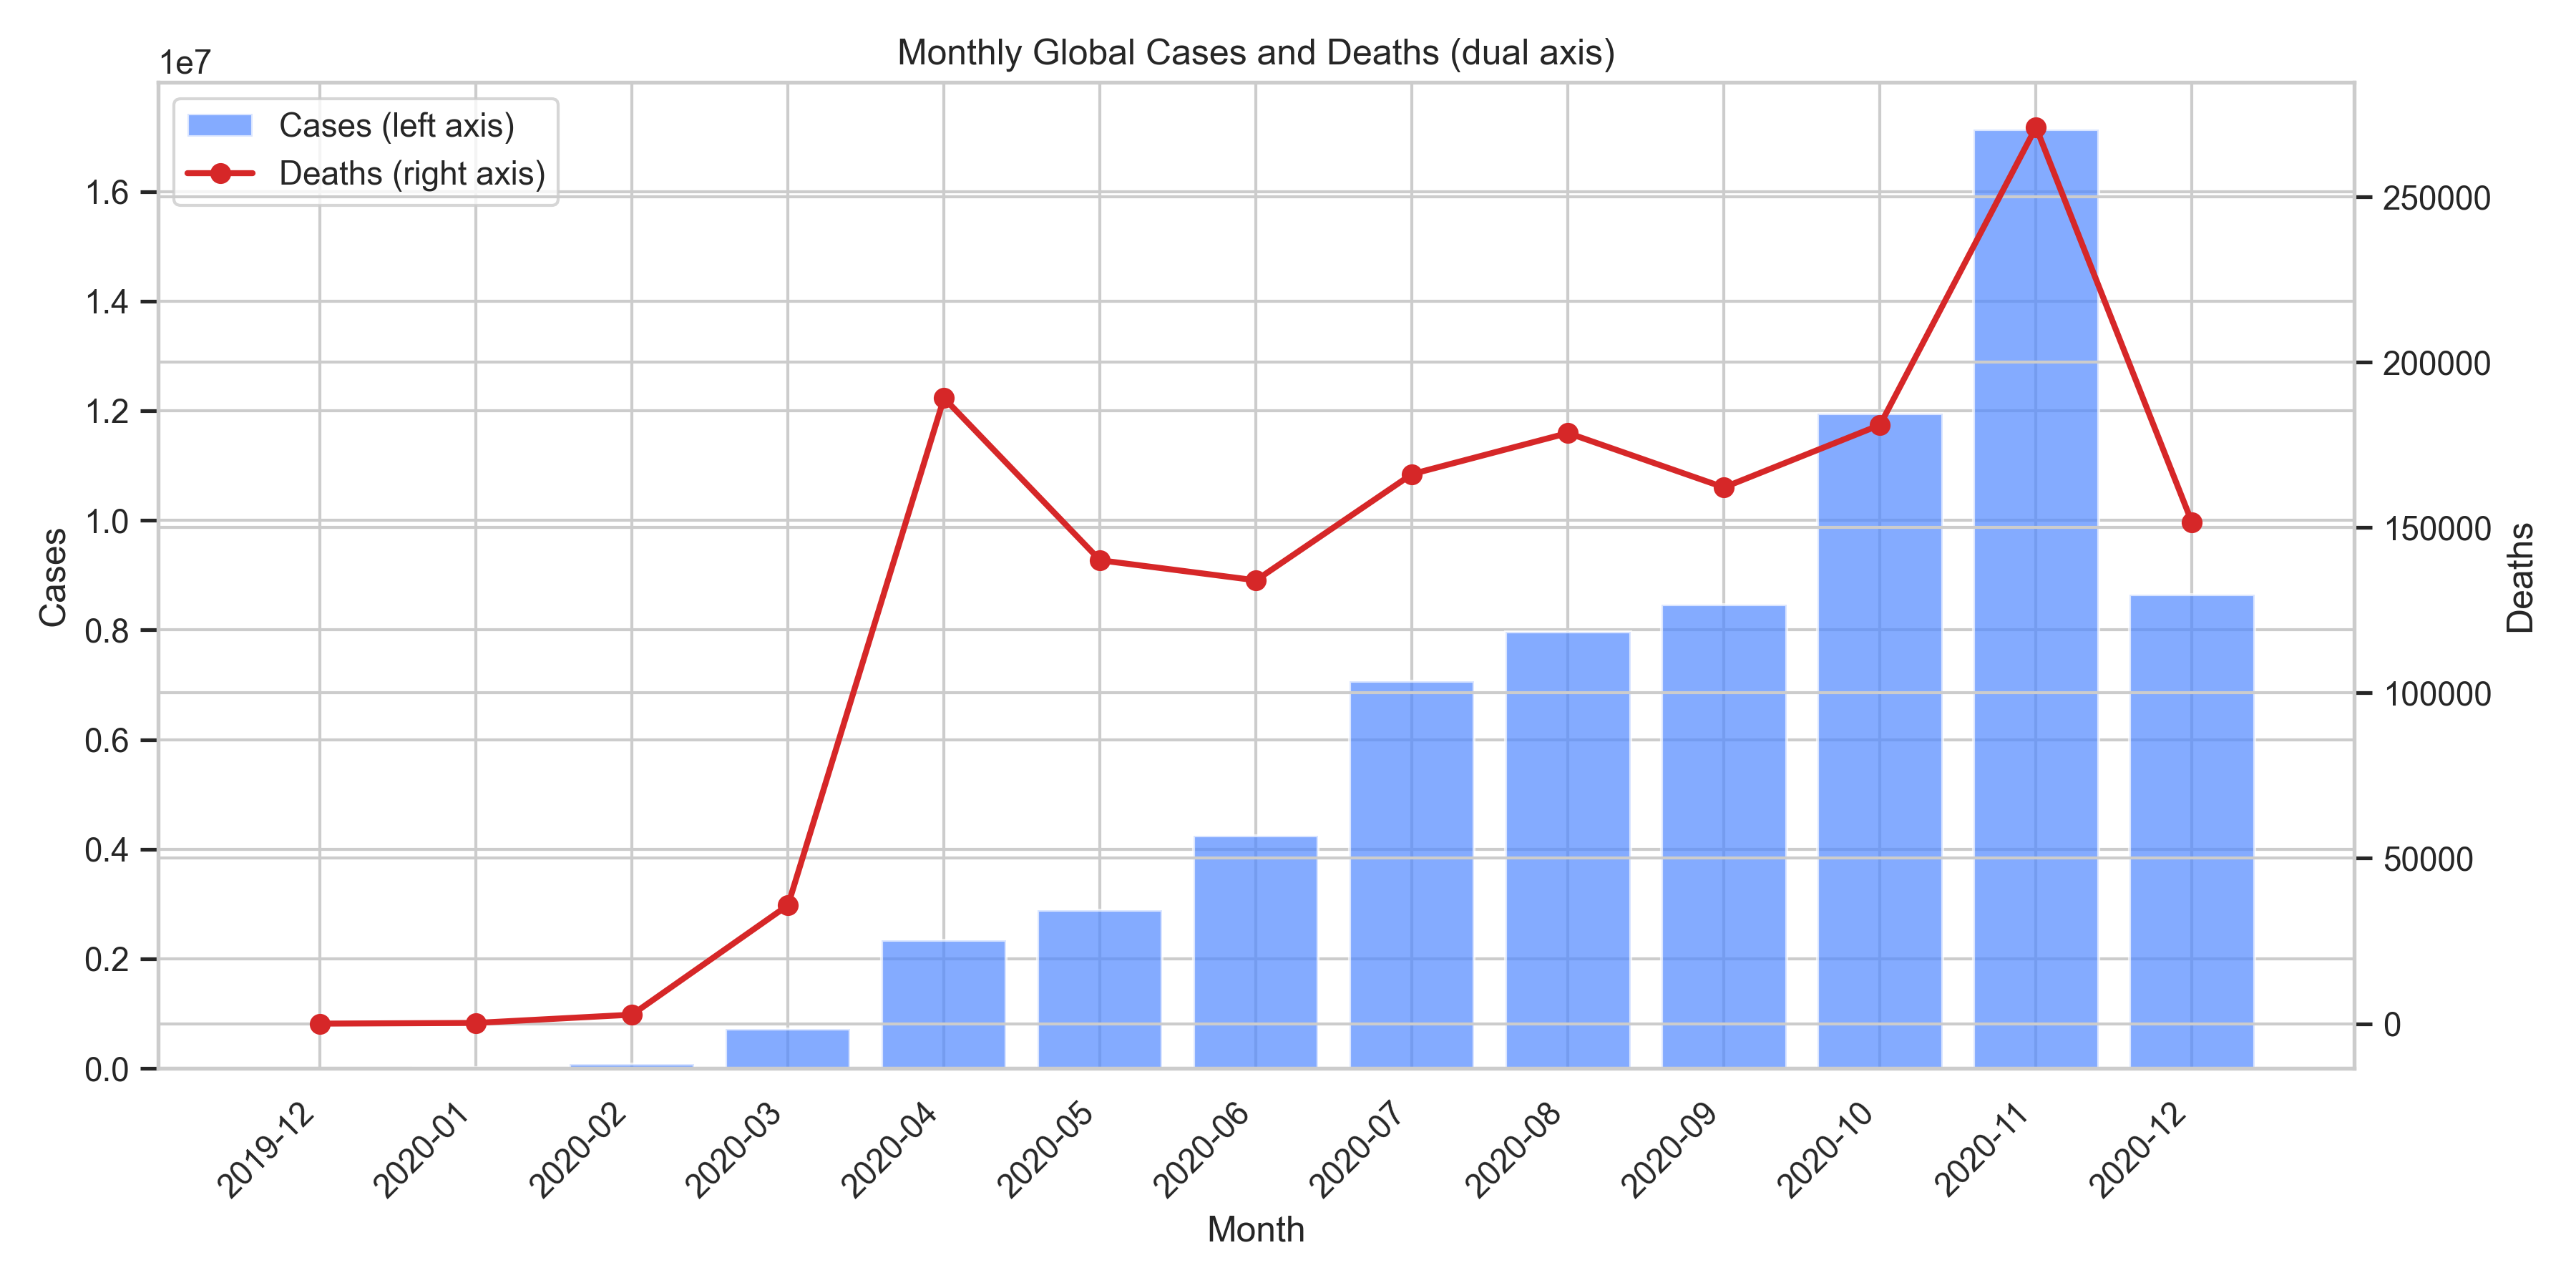
\includegraphics[width=0.85\textwidth]{monthly_trend.png}
    \caption{Monthly global cases (bars, left axis) and deaths (line, right axis). The mortality wave follows the surge in cases by roughly one month.}
    \label{fig:monthly}
\end{figure}
\FloatBarrier

\noindent Figure~\ref{fig:heatmap} operates at the country level again but focuses on intensity rather than cumulative totals. The MapReduce and Spark jobs compute rolling 14-day sums per country; the visualization script keeps only the maximum value for each territory and pivots the top 30 results into a heatmap. The palette highlights the extremes: the United States crosses 2.8 million cases over its worst 14-day window, India peaks at roughly 1.3 million, and France, Brazil, and Italy follow in the next tier. Countries lower down the list remain almost black, signaling that their surges never approached the same magnitude.
\begin{figure}[H]
    \centering
    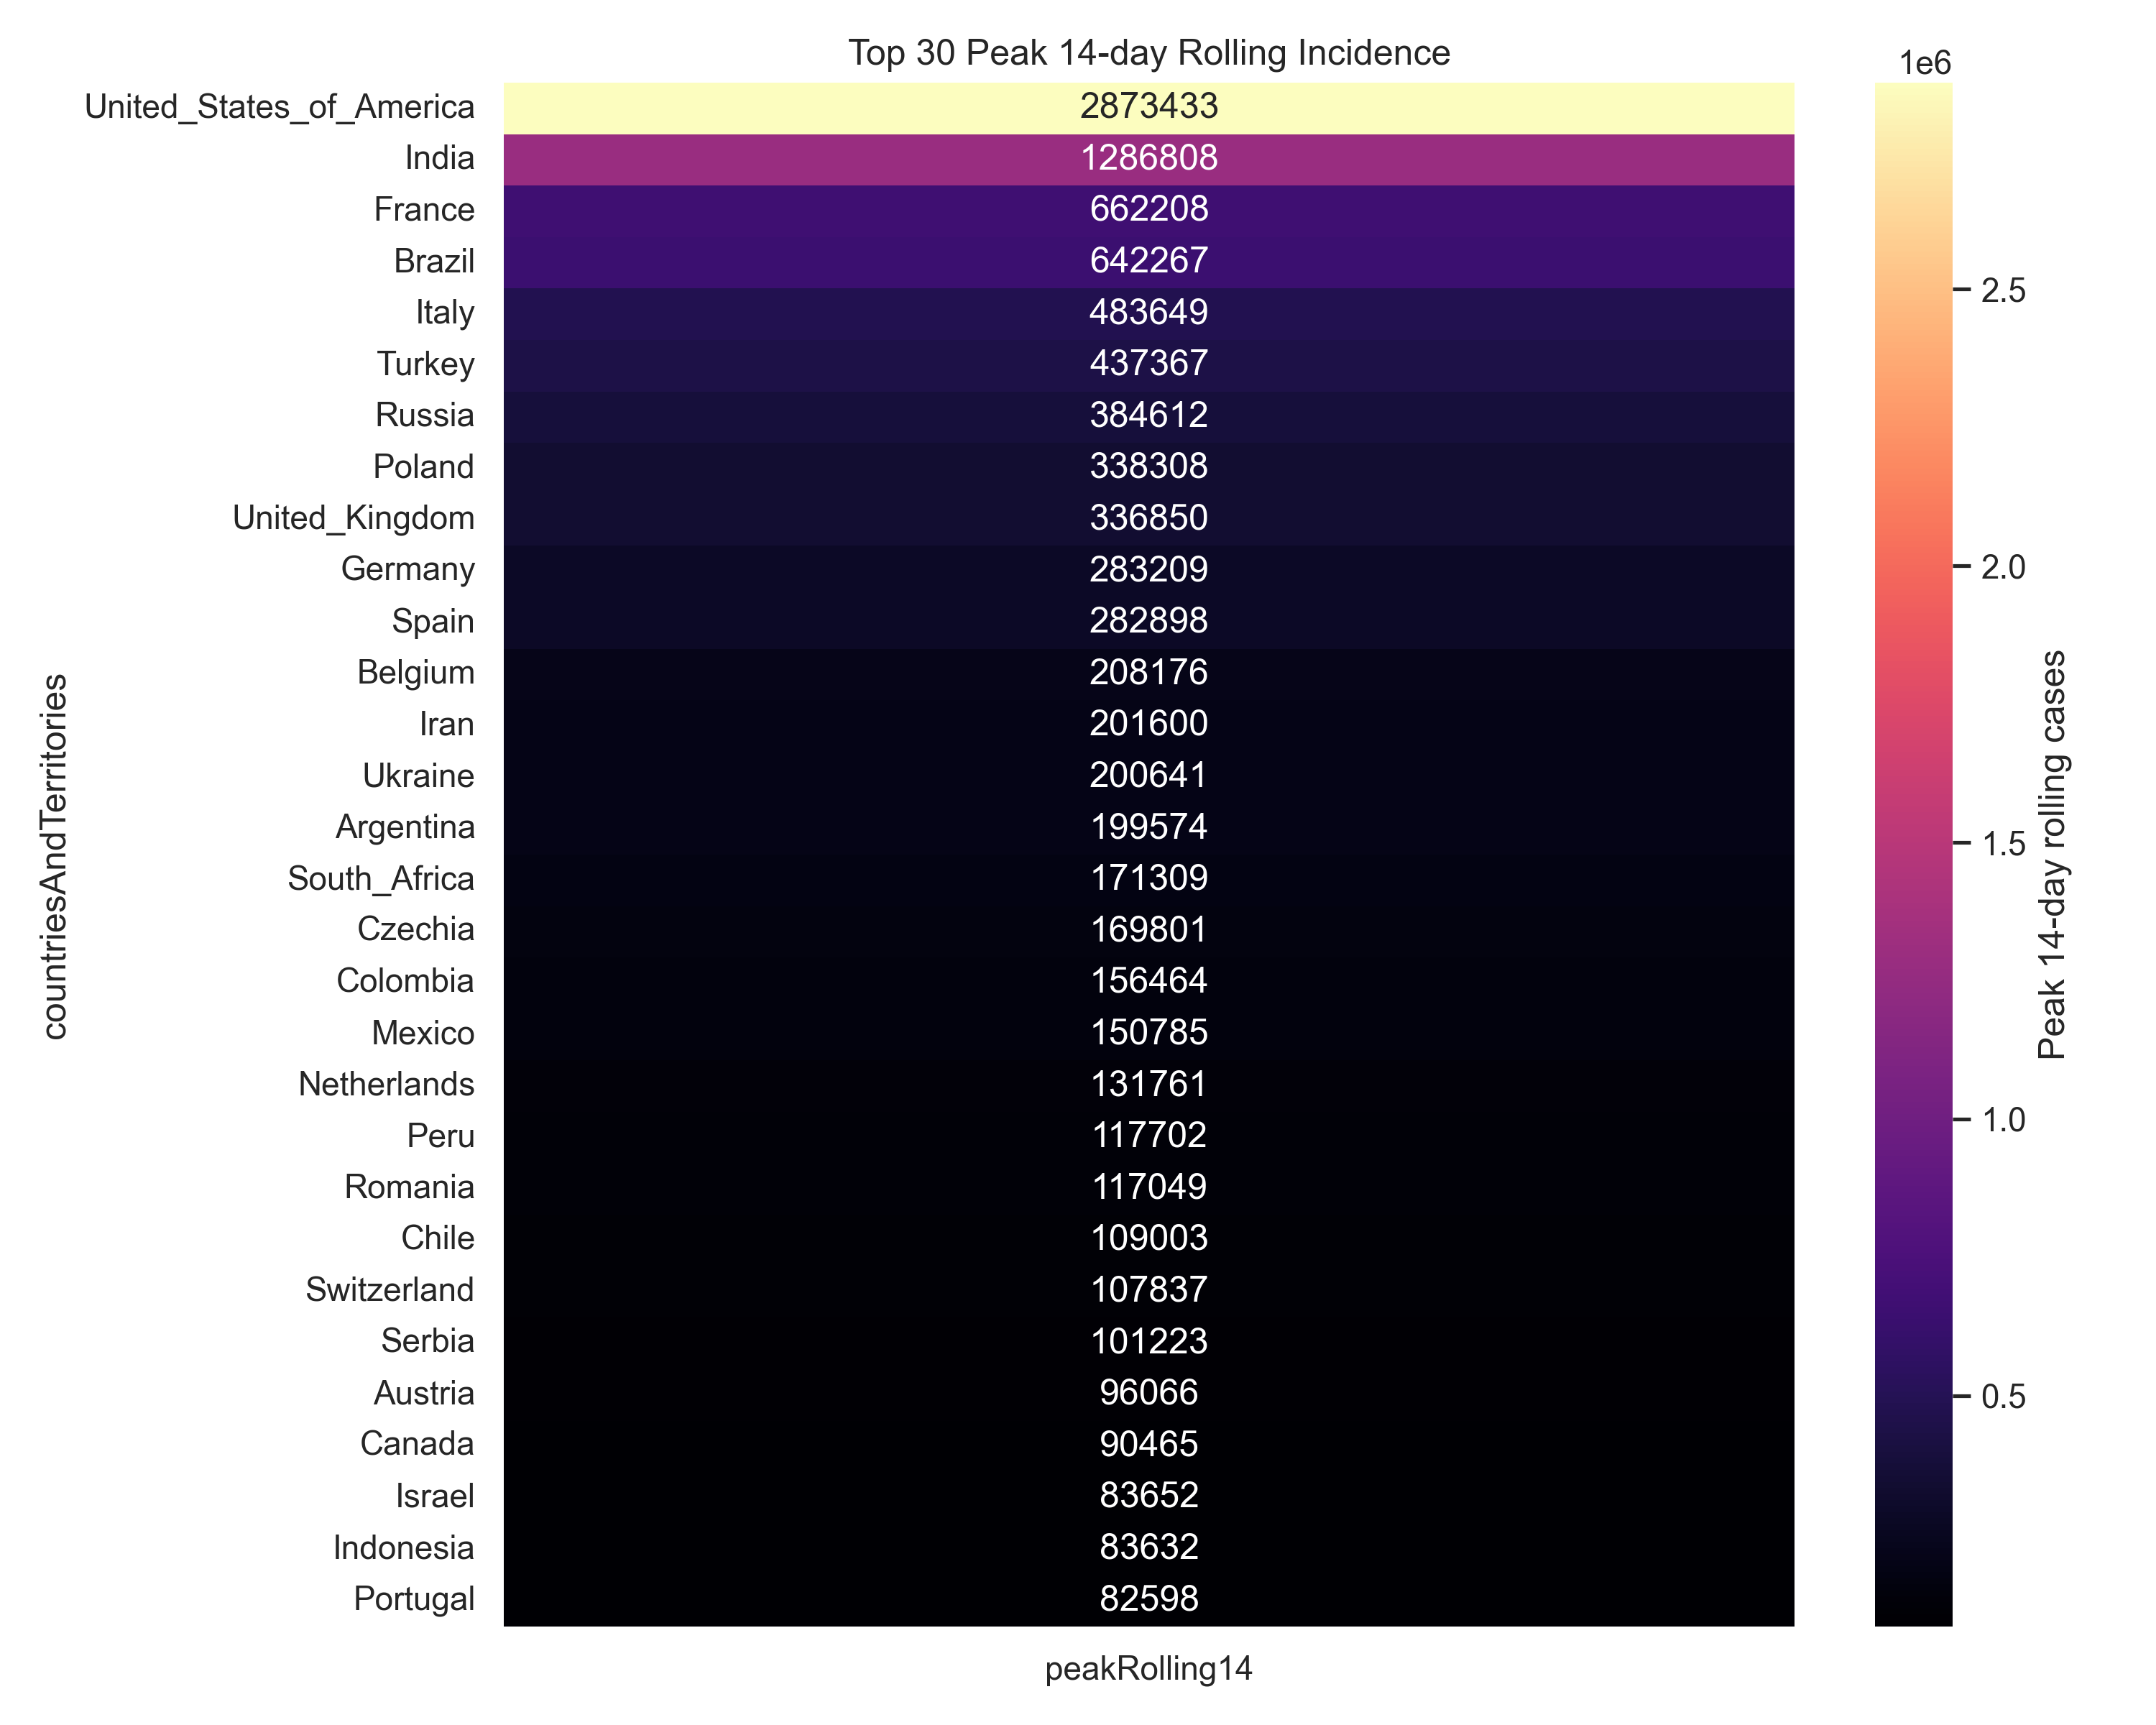
\includegraphics[width=0.75\textwidth]{peak14_heatmap.png}
    \caption{Peak 14-day rolling incidence for the top 30 territories. The colour scale emphasises the three highest peaks (United States, India, France) while the remaining countries fade toward black as their rolling totals decline.}
    \label{fig:heatmap}
\end{figure}
\FloatBarrier

Figure~\ref{fig:animation-frames} compares three snapshots of the pandemic: the quiet baseline at the end of 2019, the explosive mid-2020 surge centred in the Americas, and the widespread December~2020 phase where both hemispheres remain active. Reading the heat levels from left to right shows how quickly the epicentre shifted across continents while the gradient between low-incidence regions and global hotspots persisted.

\begin{figure}[H]
    \centering
    \begin{subfigure}[b]{0.33\textwidth}
        \centering
        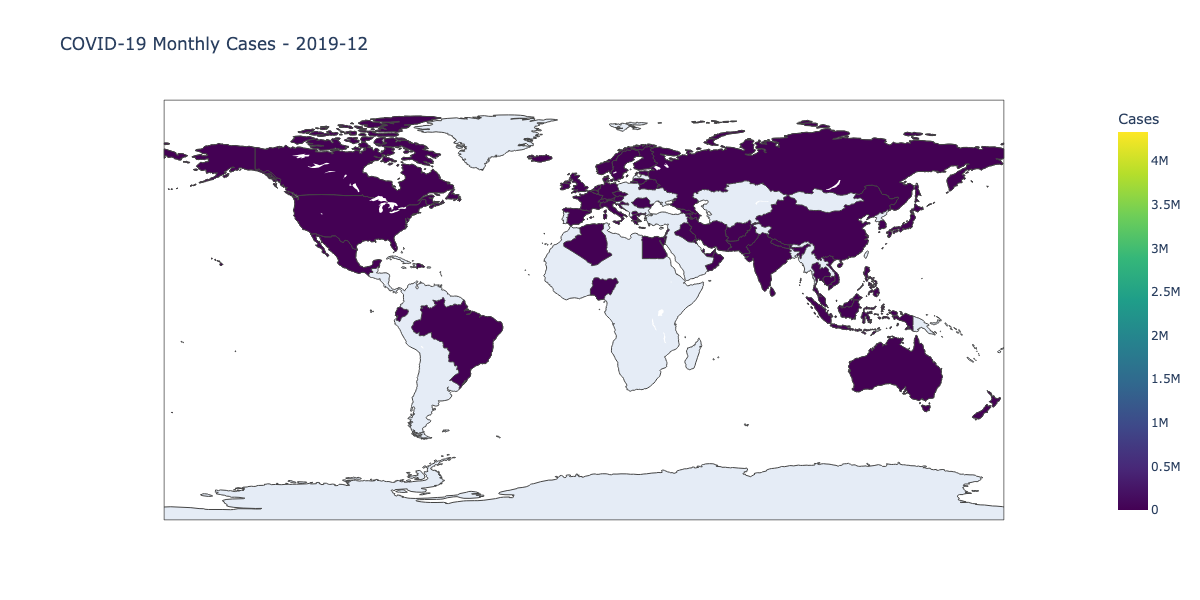
\includegraphics[width=\textwidth]{frame_initial.png}
        \caption{}
    \end{subfigure}\hfill
    \begin{subfigure}[b]{0.33\textwidth}
        \centering
        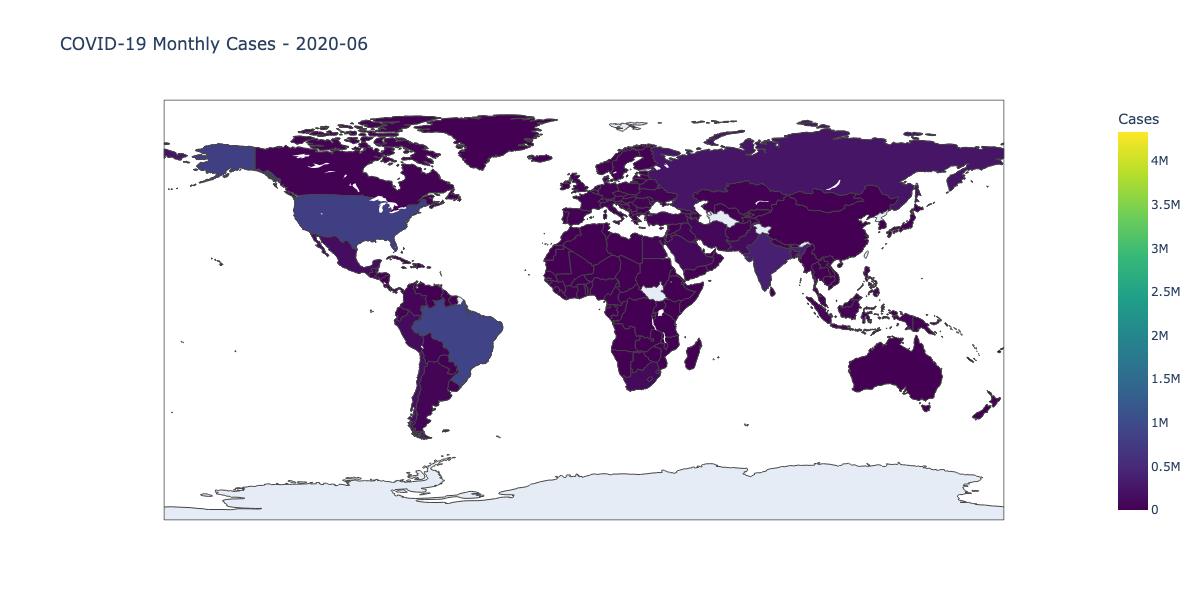
\includegraphics[width=\textwidth]{frame_peak.png}
        \caption{}
    \end{subfigure}\hfill
    \begin{subfigure}[b]{0.33\textwidth}
        \centering
        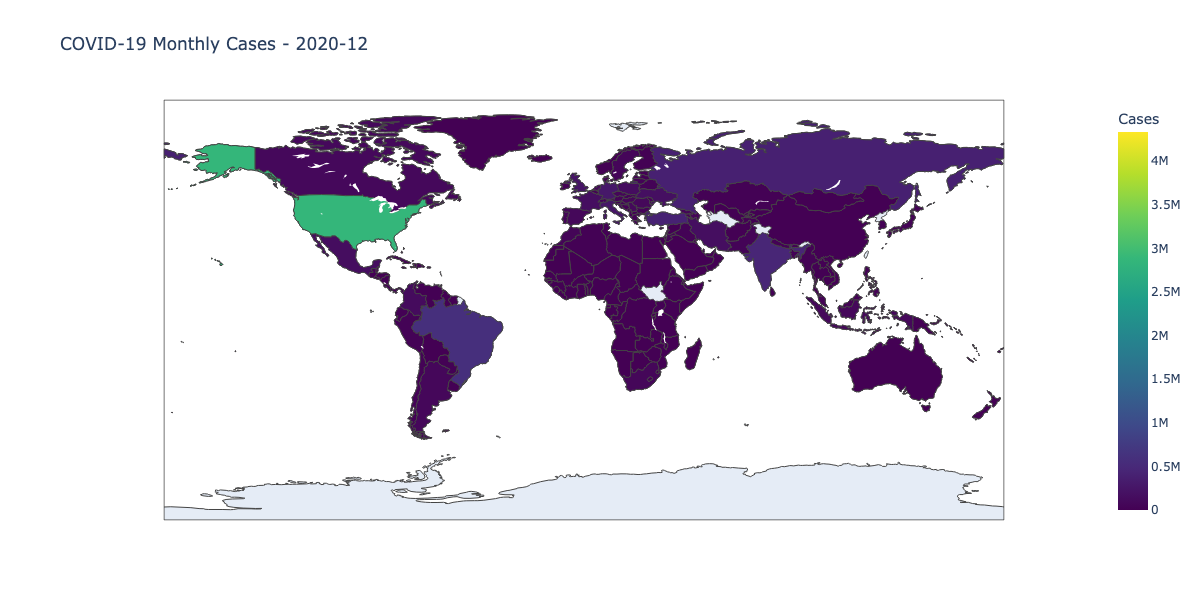
\includegraphics[width=\textwidth]{frame_final.png}
        \caption{}
    \end{subfigure}
    \caption{(a) December 2019: cases concentrated in East Asia. (b) Mid-2020: Americas become the dominant hotspot. (c) December 2020: widespread activity across both hemispheres.}
    \label{fig:animation-frames}
\end{figure}
\FloatBarrier

\noindent The full monthly animation is included in the submission (\path{Project3/visualizations/covid_animation.mp4}) and mirrored online at \href{https://github.com/raulduran/M2_GENIOMHE/blob/main/data_integration_and_big_data/Project3/visualizations/covid_animation.mp4}{this repository link}.

\section{Key indicators and performance}
\subsection{Top countries (Dec~2019 to Dec~2020)}
\begin{table}[H]
    \centering
    \caption{Top countries by cumulative cases (subset)}
    \begin{tabular}{@{}p{5.2cm}p{1.8cm}p{1.8cm}p{1.8cm}@{}}
        \toprule
        Country & Cases & CFR (\%) & Cases / 100k \\
        \midrule
        United\_States\_of\_America & 16\,256\,754 & 1.84 & 4\,940.29 \\
        India & 9\,884\,100 & 1.45 & 723.36 \\
        Brazil & 6\,901\,952 & 2.63 & 3\,270.30 \\
        Russia & 2\,653\,928 & 1.77 & 1\,819.35 \\
        France & 2\,376\,852 & 2.44 & 3\,546.86 \\
        United\_Kingdom & 1\,849\,403 & 3.47 & 2\,774.92 \\
        \bottomrule
    \end{tabular}
\end{table}
\FloatBarrier

\subsection{Performance comparison}
\begin{table}[H]
    \centering
    \caption{Average runtimes (three executions on macOS M1 Pro)}
    \begin{tabular}{@{}p{3.5cm}p{4cm}p{4cm}@{}}
        \toprule
        Engine & Job & Runtime (s) \\
        \midrule
        MongoDB MapReduce & Country totals & 0.35 \\
        MongoDB MapReduce & Peak 14-day & 0.48 \\
        Hadoop Streaming & Country totals & 1.82 \\
        Hadoop Streaming & Peak 14-day & 2.46 \\
        Spark (local[4]) & Aggregations & 2.38 \\
        \bottomrule
    \end{tabular}
\end{table}
\FloatBarrier

MongoDB proved ideal for fast exploration and quick tweaks inside the playground. Hadoop demanded more scaffolding but delivered fine-grained control that mirrors the exercises from class. Spark ran the same aggregations with compact code and produced Parquet outputs, even if the JVM start-up kept runtimes a little higher.

\newpage
\section{Discussion and conclusion}
Running the three pipelines side by side did more than stress-test the tooling. It confirmed that the underlying indicators are stable: the United States, India, and Brazil lead the global case counts, Europe faces a marked resurgence in the autumn of 2020, mortality curves trail cases by about one month, and only a handful of territories hit the most severe 14-day incidence levels. That consistency gave me confidence that each engine was wired correctly before I moved on to the next.

Each platform brought its own strengths. MongoDB offered the quickest iteration cycle, so it became the staging ground for validating calculations and exploring edge cases. Hadoop Streaming felt heavier to launch, yet it followed the exact MapReduce patterns covered in lectures, which made it a good check that I could still express the logic with explicit key-value flows. Spark sat in the middle: the codebase stayed compact, the DataFrame API kept the transformations readable, and the outputs are ready for reuse thanks to Parquet storage.

If I had more time, I would look into filling the early gaps in the case and death columns, layering in hospitalisation or vaccination context, and turning the notebook-style scripts into scheduled runs. For now, the workflow already meets the course objectives and remains faithful to the toolset we practised in class while producing a complete, reproducible study of the ECDC dataset.

\newpage
\appendix
\section*{Appendix A: Reproduce the pipeline}
\subsection*{A.1 MongoDB}
\begin{enumerate}[leftmargin=1.2cm]
    \item Launch \texttt{mongod}.
    \item Run \texttt{mongosh < MongoDB/health\_data.mongodb.js}.
    \item Export analytics with \texttt{mongoexport} if needed.
\end{enumerate}

\subsection*{A.2 Hadoop Streaming}
\begin{enumerate}[leftmargin=1.2cm]
    \item Enter the Docker container \texttt{rdurandealba/hadoop\_mac\_class}.
    \item Stage NDJSON into HDFS and make scripts executable (Section~\ref{sec:hadoop}).
    \item Run the two streaming jobs and inspect the outputs.
\end{enumerate}

\subsection*{A.3 Spark}
\begin{enumerate}[leftmargin=1.2cm]
    \item Ensure \texttt{spark-submit} is in \texttt{PATH}.
    \item Launch the job using:
\begin{lstlisting}[language=bash, caption={Spark submission helper}, float=htbp, label={lst:appendix-spark}]
spark-submit Spark/spark_health_analysis.py INPUT_FIELD GROUP_FIELD OUTPUT_DIR
\end{lstlisting}
\end{enumerate}

\subsection*{A.4 Visualisations}
\begin{enumerate}[leftmargin=1.2cm]
    \item Install \texttt{pandas}, \texttt{matplotlib}, \texttt{seaborn} (and optionally \texttt{plotly}, \texttt{ffmpeg}).
    \item Regenerate the figures and animation:
\begin{lstlisting}[language=bash, caption={Visualisation rebuild command}, float=htbp, label={lst:appendix-visuals}]
python visualizations/build_visualizations.py --input Project3/data/encounters.ndjson
\end{lstlisting}
    \item Outputs are written to \path{Project3/visualizations/outputs} (video: \path{Project3/visualizations/covid_animation.mp4}).
\end{enumerate}

\section*{Acknowledgements}
Thanks to Profesor Nazim Agoulmine for the lectures and practical sessions, and to my classmates for sharing tips about running Hadoop inside Docker on Apple Silicon.

\end{document}
